\documentclass{l4proj}
\usepackage{graphicx}
\usepackage{wrapfig}
\graphicspath{ {./images/} }
\usepackage[utf8]{inputenc}
\usepackage{enumitem}
\usepackage{comment}
\usepackage{algorithmic}
\usepackage{listings}
% \usepackage{algorithm2e}

\begin{document}

\title{Animating Network Flow}
\author{Lucy MacPhail 2183332m}
\date{February 2019}

\maketitle
%==============================================================================
%% ABSTRACT
\begin{abstract}
    The Ford-Fulkerson algorithm, used to calculate the maximum amount of flow over a network, is complex and often difficult to understand through textual means alone. This project was to create an animation of the Ford-Fulkerson algorithm for learning or teaching purposes. The animation was presented as a web application, designed to give the user as much control as possible over both the network and the playback controls to aid their understanding. When evaluated on participants having taken the Algorithmics II course, every one responded that their understanding had improved after watching the animation.
\end{abstract}

%==============================================================================

% EDUCATION REUSE CONSENT FORM
% If you consent to your project being shown to future students for educational purposes
% then insert your name and the date below to  sign the education use form that appears in the front of the document.
% You must explicitly give consent if you wish to do so.
% If you sign, your project may be included in the Hall of Fame if it scores particularly highly.
%
% Please note that you are under no obligation to sign
% this declaration, but doing so would help future students.
%
%\def\consentname {My Name} % your full name
%\def\consentdate {20 March 2018} % the date you agree
%
\educationalconsent


%==============================================================================
\tableofcontents
\chapter{Introduction}

% reset page numbering. Don't remove this!
\pagenumbering{arabic}
\section{Motivation}
\begin{comment}
Why network flow is important to learn.

Why it was important to animate it.
\end{comment}
\section{Aims}

\begin{comment}
why should I care about what are you doing and what are you actually doing?
Animating algorithms as a learning tool. [Why do people do this? What are the benefits?]
Specific algorithm: Ford-fulkerson. [What is it? Why is this algorithm important?]
Animating ford-fulkerson as a visual aid to understanding it.
\end{comment}

\chapter{Background}

\begin{comment}
what did other people do, and how is it relevant to what you want to do?

\end{comment}
\section{Network Flow}
\begin{comment}
Background of ford-fulkerson algorithm.
\end{comment}


A network is a directed graph $G=(V, E)$. There are vertices $S$ and $T$ in the set of $V$. $S$ is the source, and has no incoming edges. $T$ is the sink, and has no outgoing edges. Each edge in $E$ has a non-negative capacity.

A flow through a network $G$ must satisfy the following constraints:

\begin{itemize}[noitemsep]
    \item \textbf{Capacity constraint}: for every edge, $0 \leq flow \leq capacity$
    \item \textbf{Flow conservation constraint}: for every vertex other than $S$ and $T$, the total incoming flow must be equal to the total outgoing flow.
\end{itemize}

\begin{figure}[h]
    \centering
    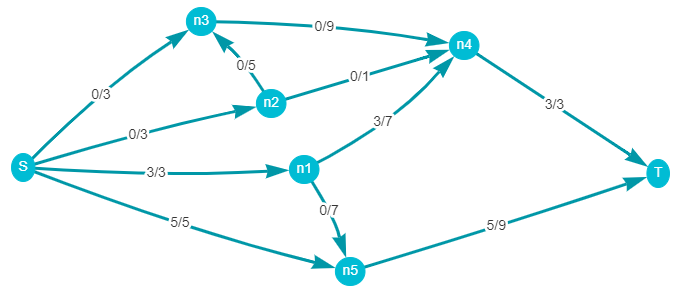
\includegraphics[width=0.9\textwidth]{network-example.png}
    \caption{An example of a network, with a flow of 16. Each edge has a label of the format $x/y$, where $x$ is the flow through the edge and $y$ is the capacity of the edge.}
    \label{fig:network}
\end{figure}

\subsection{Augmenting path}
An augmenting path is a path from $S$ to $T$, comprised of the edges of $G$ but not necessarily directed as in $G$. Each edge (u,v) in the path must satisfy one of the two following conditions:

\begin{enumerate}
    \item $(u,v) \in E$, and $f(u,v) < c(u,v)$. This is a forward edge, and the different $c(u,v) - f(u,v)$ is referred to as the slack of $(u,v)$
    \item $(v,u) \in E$, and $f(u,v) > 0$. This is a backward edge.
\end{enumerate}

\begin{figure}[h]
    \centering
    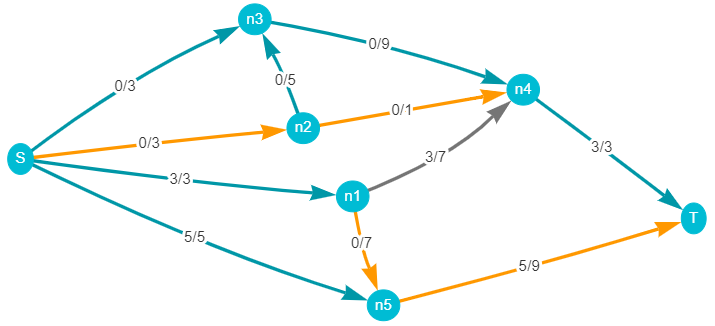
\includegraphics[width=0.9\textwidth]{aug-path-example.png}
    \caption{An augmenting path through the graph shown in Figure \ref{fig:network}. Forwards edge are shown in orange, and backwards edges in grey.}
    \label{fig:aug-path}
\end{figure}

The \textbf{Augmenting Path Theorem} states that a flow along a network is maximum if and only if the network admits no augmenting path.

\subsection{Residual graph}
We have that $G=(V,E)$ is a network with capacity function $c$, and $f$ is a flow through $G$. Then the residual graph $G'=(V',E')$ with respect to $G$ and $f$ is a directed graph with capacity function $c'$. $G'$ has the same set of vertices as $G$, $V'=V$.

$(u,v) \in E'$ if and only if:
\begin{itemize}
    \item $(u,v) \in E$ and $f(u,v)<c(u,v)$. In this case, $c'(u,v) = c(u,v) - f(u,v)$. This is a \textbf{forwards edge.}
    \item $(v,u) \in E$ and $f(u,v)>0$. In this case, $c'(u,v) = f(v,u)$. This is a \textbf{backwards edge}.
\end{itemize}

A directed path through the residual graph $G'$ from $S$ to $T$ corresponds to an augmenting path in $G$.

\begin{figure}[h]
    \centering
    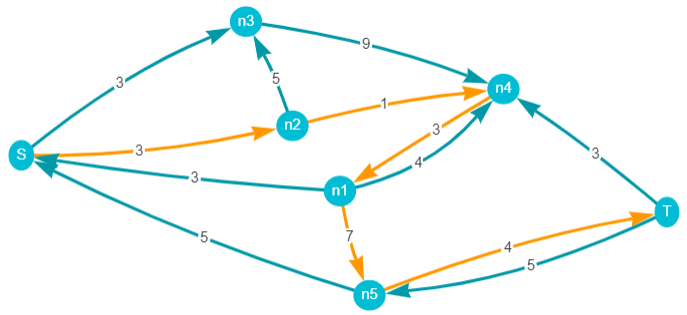
\includegraphics[width=0.85\textwidth]{res-graph-example.png}
    \caption{The residual graph of the above network. The path from $S$ to $T$ corresponds to the augmenting path from Figure \ref{fig:aug-path}.}
    \label{fig:my_label}
\end{figure}

\subsection{Minimum cuts}

\begin{figure}[h]
    \centering
    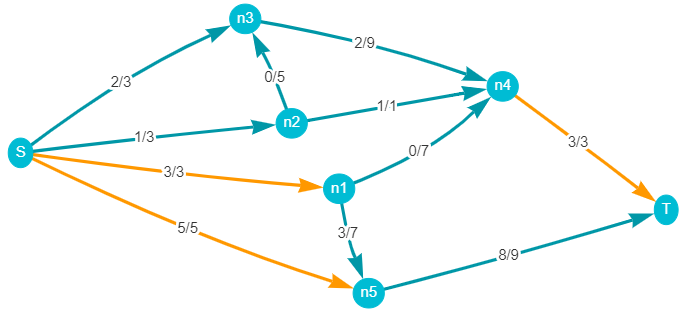
\includegraphics[width=0.85\textwidth]{min-cut-example.png}
    \caption{The residual graph of the above network. The path from $S$ to $T$ corresponds to the augmenting path from Figure \ref{fig:aug-path}.}
    \label{fig:my_label}
\end{figure}

\subsection{Ford-Fulkerson}



\section{Algorithm Animation}

\begin{comment}
Teaching algorithms using a visual aid; research into that. Leads into...

\end{comment}
\chapter{Analysis/Requirements}
For the product to be used in an educational context, it was decided that it should be designed as a web-based application. This would mean that it would be easily accessible and distributed.
\section{Analysis of Similar Examples}
The only example of a web application animating network flow that could be found was on the site visualgo.net \cite{visualgo}.
\begin{figure}[h]
    \centering
    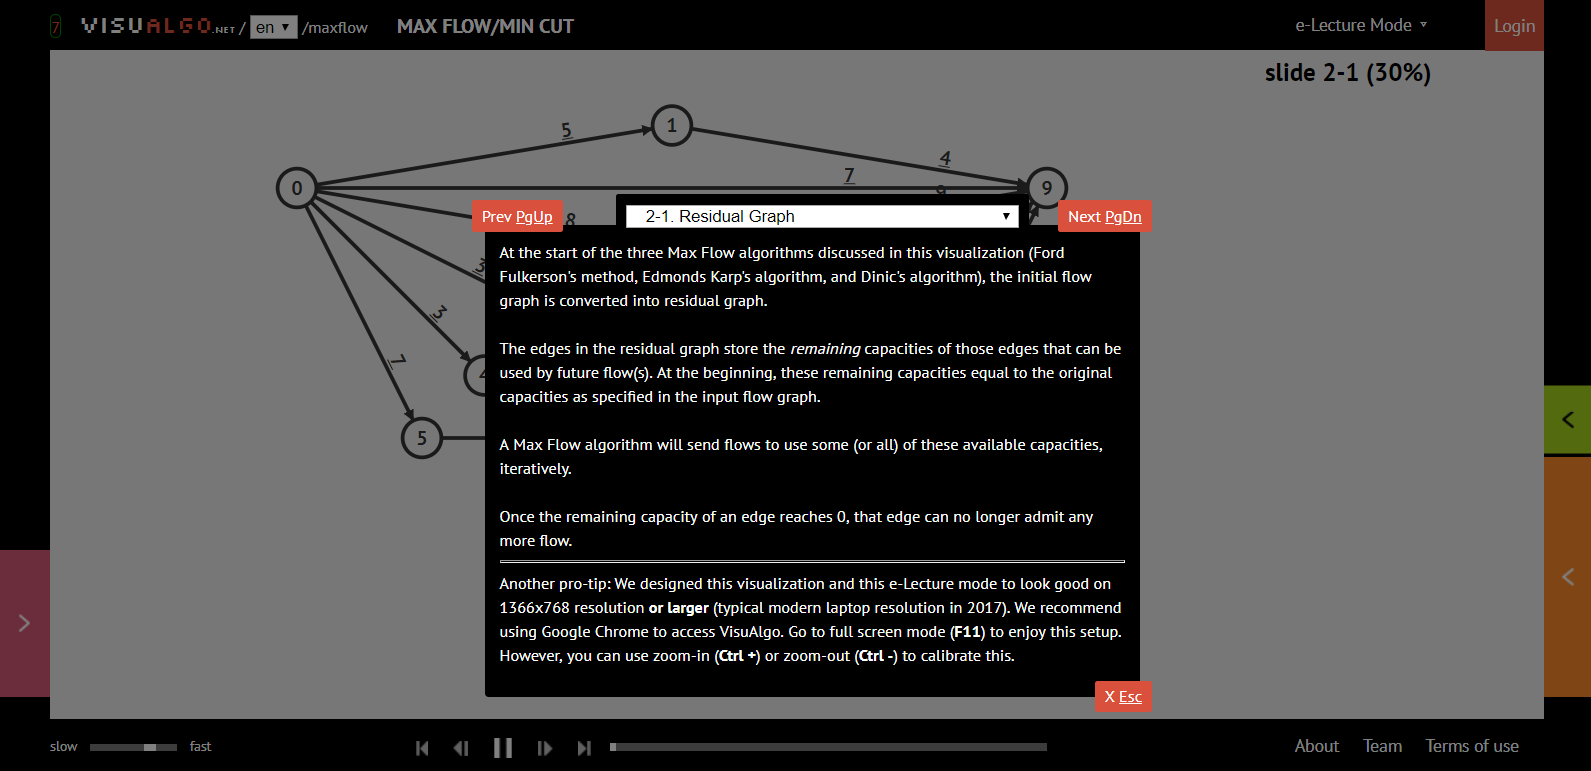
\includegraphics[width=\textwidth]{visualgo1.png}
    \caption{The first screen shown to the user when the user opens the algorithm. Lecture notes describing what you can see overlay over the graph, until closed.}
    \label{fig:my_label}
\end{figure}

To interact with the application, the user must open the pink tab in the lower left corner. This allows them to select the method of network flow (Ford-Fulkerson being one of the options), and which nodes are the Source and the Sink node.
\begin{figure}[h]
    \centering
    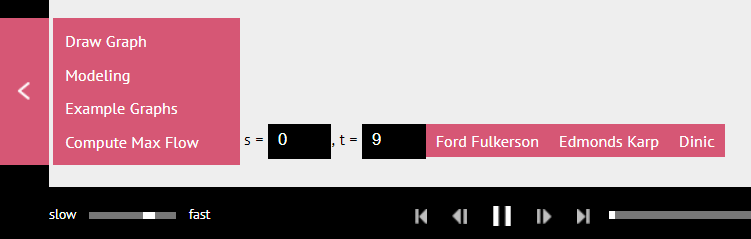
\includegraphics[width=0.8\textwidth]{visualgo2.png}
    \caption{The overlay to choose calculate the algorithm.}
    \label{fig:my_label}
\end{figure}

There were additional overlays on the right-hand side of the application. One (yellow) printed out the action that the animation was executing, and another (orange) had a pseudo-code panel which highlighted the line that was being executed at each point in the animation.

\begin{figure}[h]
    \centering
    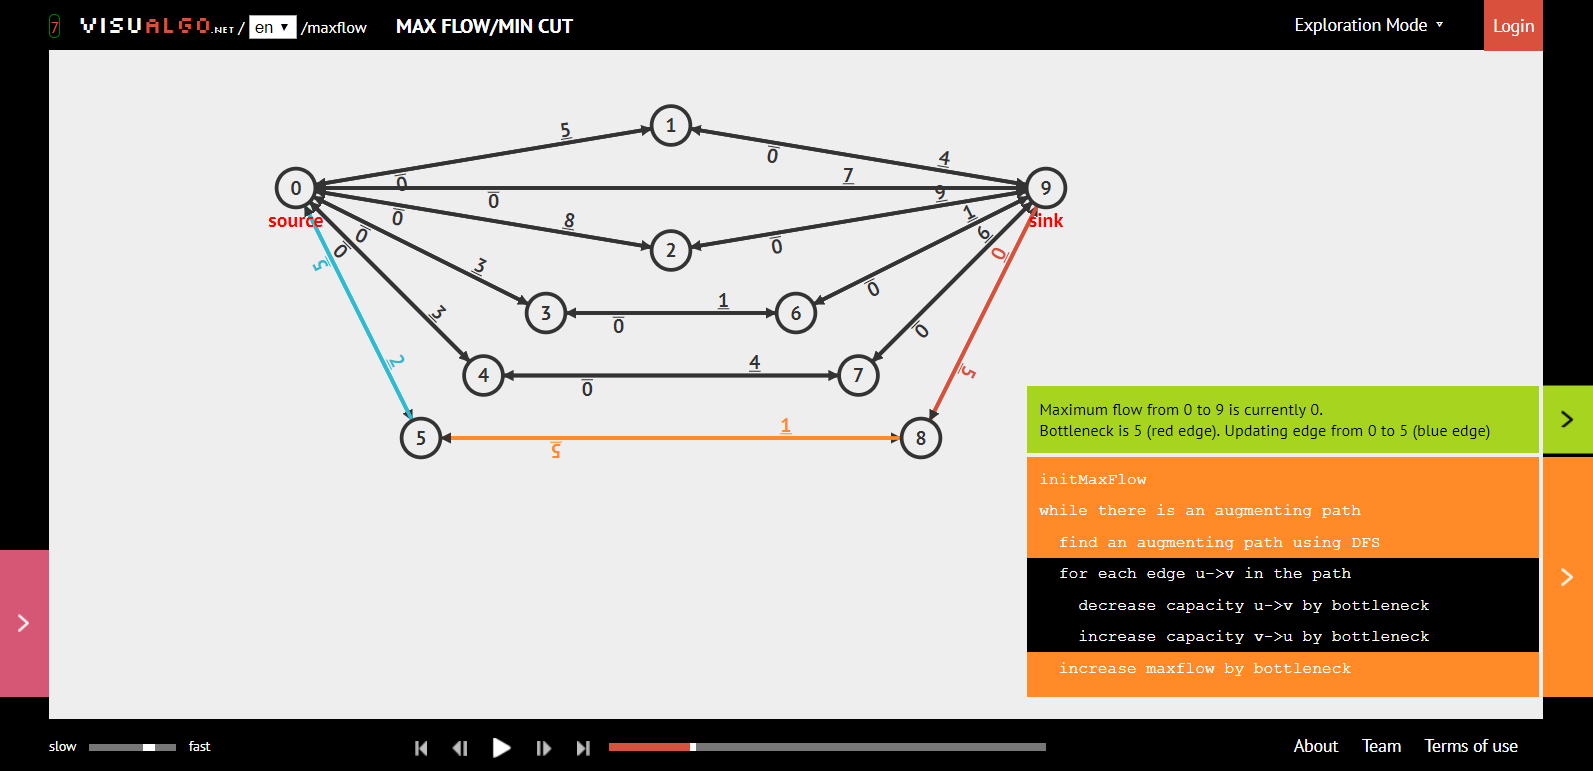
\includegraphics[width=\textwidth]{visualgo3.png}
    \caption{The animation, part-way through execution.}
    \label{fig:my_label}
\end{figure}

Some of the positive aspects of this example:
\begin{itemize}[noitemsep]
    \item The layout devoting the large central portion of the screen to the animation
    \item The slide out features on either side of the screen provided a sensible level of information, without interfering with the display of the animation.
    \item The playback controls, with the options to step forward, backward, and change the speed of animation.
    \item The progress bar (bottom-middle), as the user could drag it forward and back to see different points of the animation.
    \item The user could pick example graphs which make the algorithms act in a particular way, or draw their own.
    \item The choice of a particular network flow algorithm, in addition to Ford-Fulkerson.
\end{itemize}

However, this example presented a lot of opportunities for improvement:
\begin{itemize}[noitemsep]
    \item The initial slides at the beginning were a text-heavy way to convey information, where an animated algorithm should try and use graphical means to teach. The application also relied on these slides to teach the user how to interact it.
    \item The layout of the graph was confusing, as each edge has an number upside-down. Not only is this harder to read, but it is not clear what the numbers represent.
    \item The lack of the residual graph, which is a powerful graphical tool for teaching the Ford-Fulkerson algorithm.
    \item The animation is very confusing, such that even a person highly familiar with the algorithm has difficulty determining what it is doing.
    \item Many bugs and usability issues. The drawing feature allows easy addition of nodes and edges, but no clear control with creating the weights of edges.
\end{itemize}

In general, visualgo provided a lot of features which could be really effective for teaching network flow, but executed them poorly.

As no other examples of network flow animation could be found, other algorithm animation web applications were found which involved networks. The first of these was algomation.com \cite{algomation}, which hosts a large variety of algorithms as well as provides the ability for users to create or fork them. The algorithm in this example is Prim's Minimum Spanning Tree, as it also uses a network.

\begin{figure}[h]
    \centering
    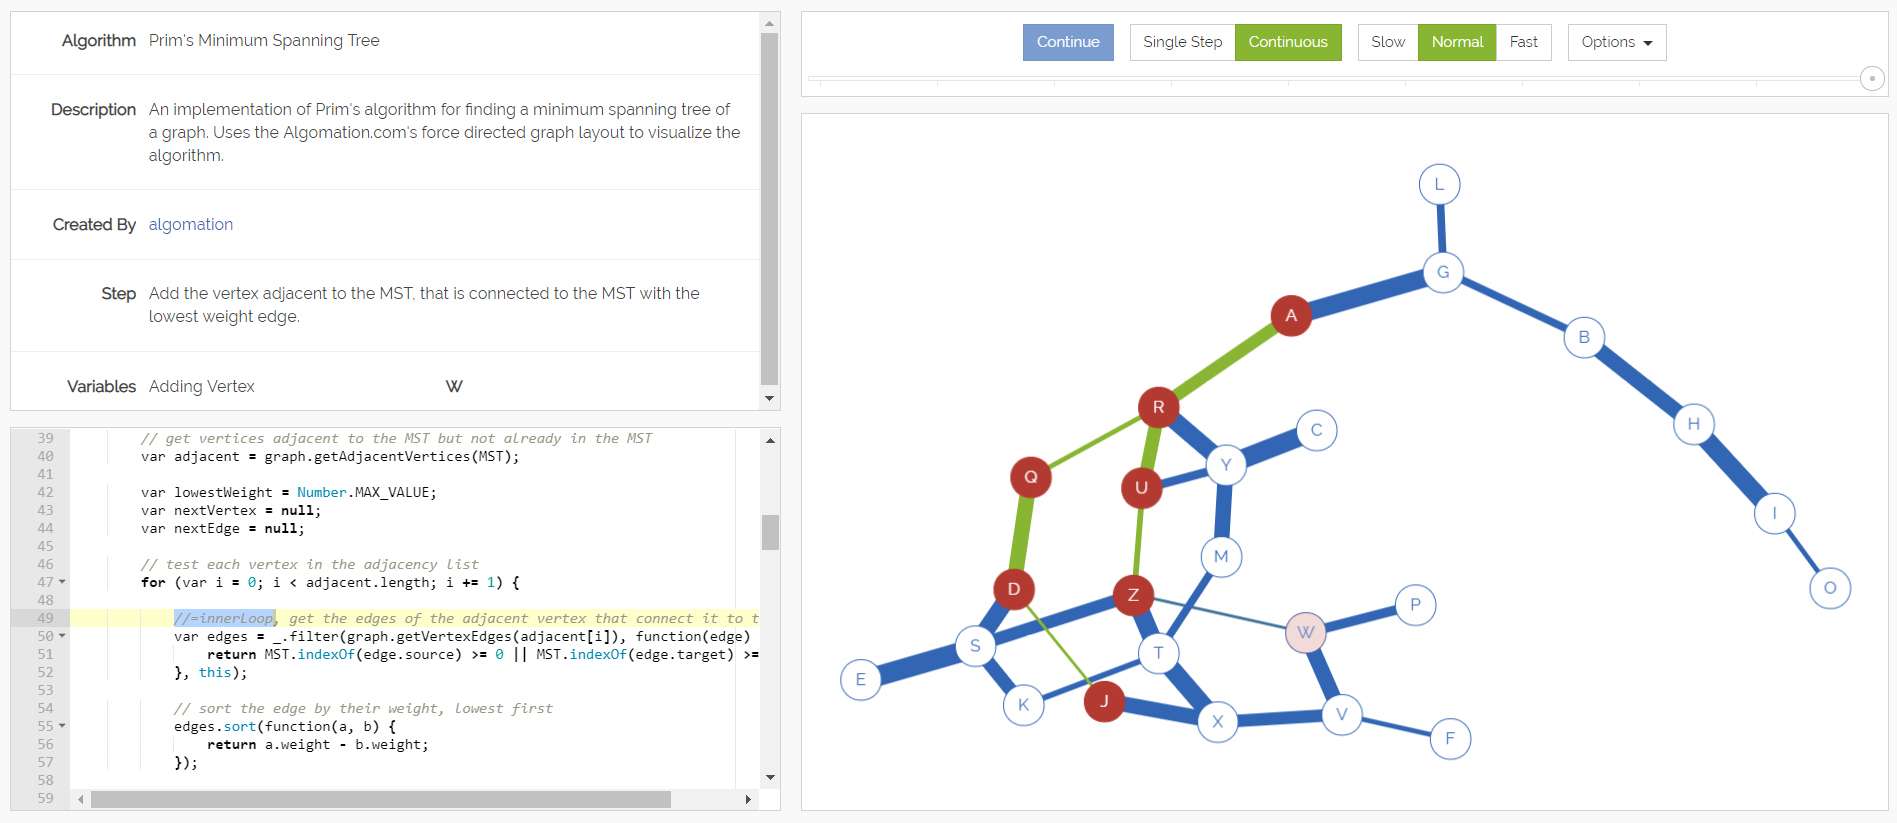
\includegraphics[width=\textwidth]{algomation1.png}
    \caption{Algomation's representation of Prim's Minimum Spanning Tree}
    \label{fig:my_label}
\end{figure}

The positive aspects of algomation included:
\begin{itemize}[noitemsep]
    \item Smooth and clear diagrams and animation
    \item Concise description of algorithm (top-left), avoids unnecessary information and assumes user has some knowledge.
    \item Clear and intuitive playback controls. Similarly to visualgo there is a progress bar, but here it expands as the animation runs. Once animation is complete, the user can drag the progress bar back and forth.
    \item Describes step of algorithm and relevant variables. Jumps to current place in code throughout animation.
    \item The user may select one of three speeds for the animation to run.
\end{itemize}

Some aspects of Algomation's design weren't ideal for this project, however:
\begin{itemize}[noitemsep]
    \item The graph was not customisable in any way.
    \item The use of the algorithm's source code on the bottom left is perhaps too detailed for the purposes of the project.
    \item The step and variable sections of the data that updated for each stage of the algorithm did not draw the eye when they changed. This was useful information that could have been made more obvious.
\end{itemize}
Each feature of Algomation was clean and well executed, but did not include enough for the ideal outcome of this project.

Another example of animated algorithms included in research was a website run by David Galles from the Computer Science department of the University of San Fransisco \cite{usfca}. Once again, there was no example of network flow but a different network related algorithm was chosen, the Breadth-First Search path finding algorithm.

\begin{figure}
    \centering
    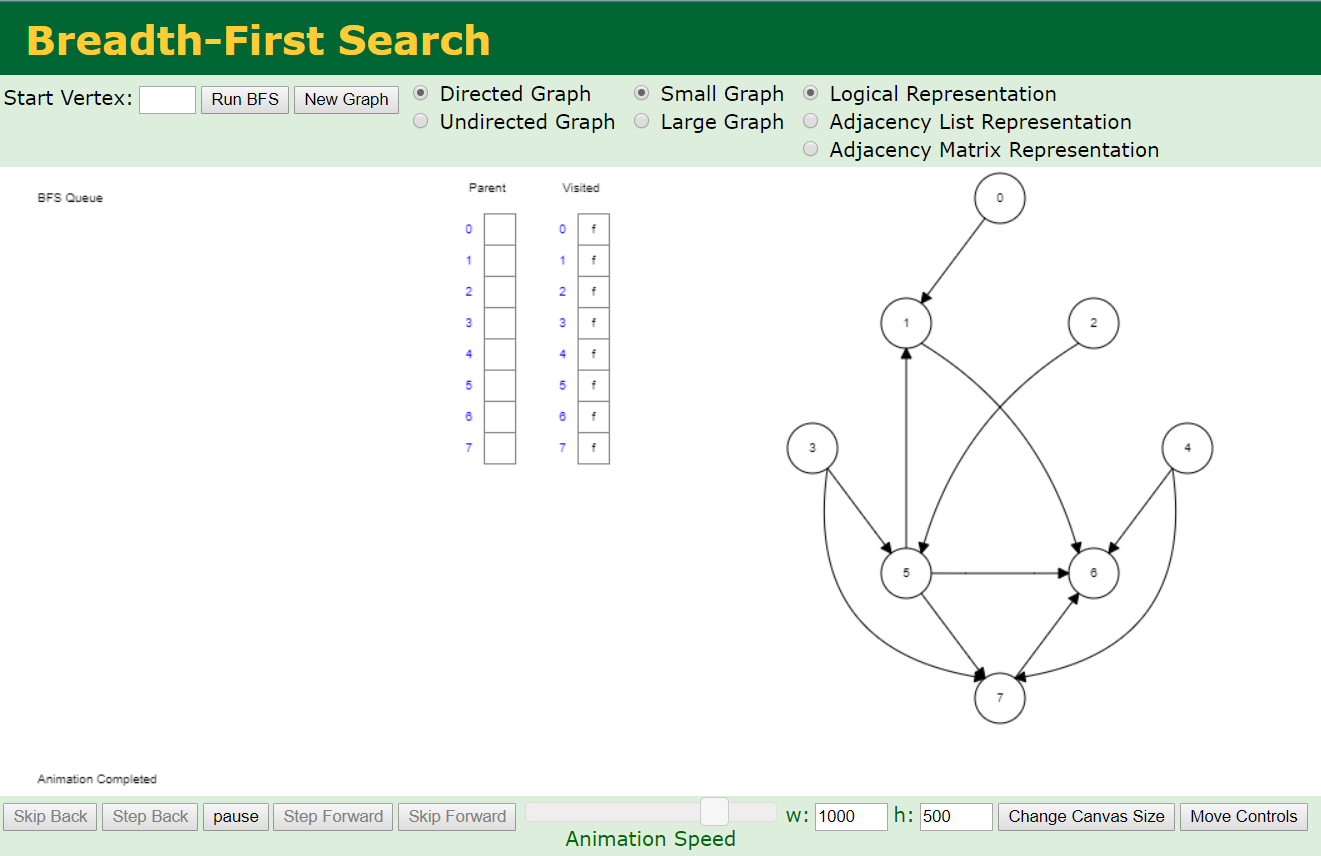
\includegraphics[width=\textwidth]{usfca1.png}
    \caption{The USFCA representation of the BFS}
    \label{fig:my_label}
\end{figure}

The features that were positive included:

\begin{itemize}[noitemsep]
    \item Clear, randomly generated graphs, with options for small or large.
    \item Easy to use playback controls with speed control.
    \item Additional information for the algorithm presented in a clear manner.
    \item Sensible interface, each feature works as expected.
\end{itemize}

However the layout of the web page detracts from the animation. The middle section is divided into 3 equal sections, where only the graph off to the side fills up its entire space. Using the "Change Canvas Size" controls in the bottom doesn't affect the size of the objects on the screen, just the screen itself, which makes this feature feel redundant.

The lack of animations for network flow algorithms showed that they are challenging to visualise effectively. There are many different aspects of the algorithm to consider, and the graphical animation alone is not enough to communicate the algorithm to the user.

\section{List of requirements}
Taking each of the different examples into consideration, a list of fundamental requirements for the project was devised.

\begin{itemize}[noitemsep]
    \item \textbf{A clear, readable graph}, including few edge overlaps, a large canvas size, and clear labels on edges. This is so that the display of the graph won't obscure crucial information conveyed during the animation.
    \item \textbf{Playback controls} of start, stop, speed up/down, and move forwards/backwards. This allows a user to traverse through the animation at their pace, whether teaching or learning from the algorithm.
    \item \textbf{The ability of a user to generate or draw a graph}. If the user has greater control over the network used in the animation, it means they can display certain cases of the algorithm, or use familiar cases to learn from.
    \item \textbf{Information on each step of the algorithm during its execution} including pseudo-code of the algorithm.
    \item \textbf{Intuitive interface}, so that the user isn't distracted from the main point of the application by struggling to effectively use it.
\end{itemize}

\chapter{Design}

\section{Network generation}
A fundamental requirement of the tool is the user's ability to generate a network in multiple different ways. Someone teaching the Ford-Fulkerson algorithm may want to display a specific network, which exhibits a rarer case of the algorithm during execution. For variety, a user may want a randomly generated network if aiming for a more general understanding of the algorithm.

Two of the network creation methods require very little input from the user. The simplest is a default network taken from the Algorithmics II teaching notes. This exhibits a case of a backwards edge being decremented, and is a consistent option for the user. The random generation takes the desired number of nodes in the graph, and will draw a randomised network with node $S$ on the far left and node $T$ on the far right side of the screen. Further information on the implementation of this is provided in section \ref{randomise}.

\begin{figure}[h]
    \centering
    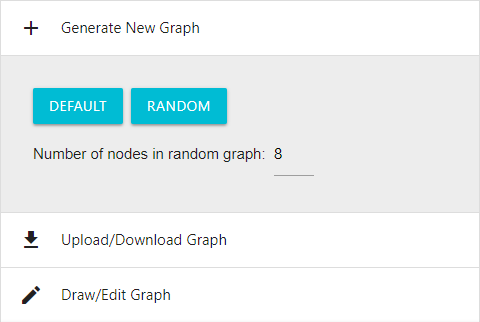
\includegraphics[width=0.5\textwidth]{graph-gen-tools.png}
    \caption{The menu for network generation tools.}
    \label{fig:my_label}
\end{figure}

If the user desires greater control over the graphs, the design includes additional network creation methods. The first of these features allowed the user to download or upload a file with a representation of the graph on it. This can be used to save randomly drawn graphs that may serve as good teaching examples to use later.

The second is a drawing feature, in which the user may directly interact with the canvas and create networks of their own design. This raised issues, as there were a variety of potential ways in which a user could add nodes and edges to join them. Not only this but the nodes $S$ (the source node) and $T$ (the sink node) had to be included in the network, in positions consistent with the other networks created. The final design of the drawing feature included the following features:
\begin{itemize}[noitemsep]
    \item Once the drawing mode was activated, $S$ and $T$ would be displayed in set positions at the left and right of the screen, so that the user could add as many nodes in-between as required.
    \item To interact with the canvas there would be a toolbar at the top with two buttons, ``add node" and ``add edge".
    \item When ``add node" is selected the user can click to place one node anywhere on the screen, or cancel the action. The nodes are labelled ``$n1, n2, n3... nx$" in the order that they are placed in.
    \item When ``add edge" is selected, the user may drag an edge from one node to another. Once two nodes are connected, the user is prompted to choose a capacity (default 4), such that if `$x$' is entered, the new edge's label is ``$0/x$".
    \item When any node or edge is selected, a third button appears in the toolbar to ``delete selected". If a node is deleted, it is removed from the graph along with any edges connected to it. The user may delete any node except for $S$ or $T$.
    \item The user may not connect a node to itself, or enter a capacity that is not an integer, but there are very little other restrictions. It is assumed that if the user wishes to draw a graph that could not possibly run the Ford-Fulkerson algorithm, they have some reasoning behind it.
\end{itemize}

\section{Additional Information}
The graphical element of the algorithm would not be enough alone to convey a meaningful amount of knowledge to the user. Therefore a pseudo-code panel, execution trace section, and flow counter panel were added, to be updated at different stages of the animation.
\subsection{Pseudo-code}
The pseudo-code panel contained a broad description of the algorithm. As different sections of the algorithm were executed in the animation, the corresponding line of the pseudo-code would be highlighted.

\begin{figure}[h]
    \centering
    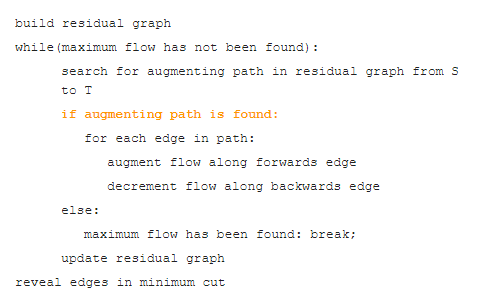
\includegraphics[width=0.6\textwidth]{pseudocode1.png}
    \caption{The pseudo-code panel, midway through an animation.}
    \label{fig:my_label}
\end{figure}

\subsection{Execution Trace}
The execution trace is a section which prints a new line after each significant action is completed in the animation. For example, during the building of the residual graph, the execution trace will print ``adding a forwards/backwards edge of capacity x" for each edge. Or if the algorithm is currently searching for an augmenting path, the latest line will be ``Searching for augmenting path..." and subsequently ``augmenting path found: 0, x, y, z, T".

\begin{figure}[h]
    \centering
    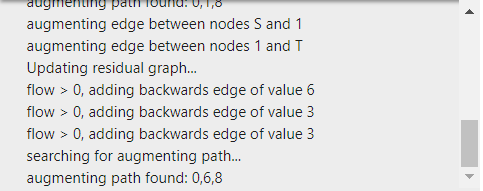
\includegraphics[width=0.6\textwidth]{traceback.png}
    \caption{The execution trace during an animation.}
    \label{fig:my_label}
\end{figure}

\subsection{Flow Counter}
After each iteration of the algorithm, the flow counter will update to match the current amount of flow passing through the network. By the end of the animation, it will contain value of the maximum flow.

\section{Playback Controls}
An end goal of the project was to have controls to play, pause, change the speed, or move step-wise through the algorithm. Therefore, the design included 4 playback buttons used to rewind, step backwards, play/pause (toggle), or step forwards. Additionally a speed control slider was included, which affected the speed of the animation both forwards and backwards.

\begin{figure}[h]
    \centering
    
\includegraphics[width=0.45\textwidth]{playback1.png}
    
\includegraphics[width=0.48\textwidth]{playback2.png}
    \caption{The playback buttons, and the speed control slider while being adjusted}
    \label{fig:my_label}
\end{figure}

To avoid the use of needless written instructions where possible, the use of the tortoise and the hare icons were used to indicate the purpose and direction of the speed control slider.

\section{Layout}
Similar examples to this project all shared a common layout theme; a canvas taking up a large portion of the screen would contain the animated network, with supplementary information in containers off to the side or top of the main canvas. The product was designed to fit entirely on one web page, with the graphs taking up three quarters of the screen, and the remaining portion dedicated to a information bar on the left.

\begin{figure}[h]
\centering
\fbox{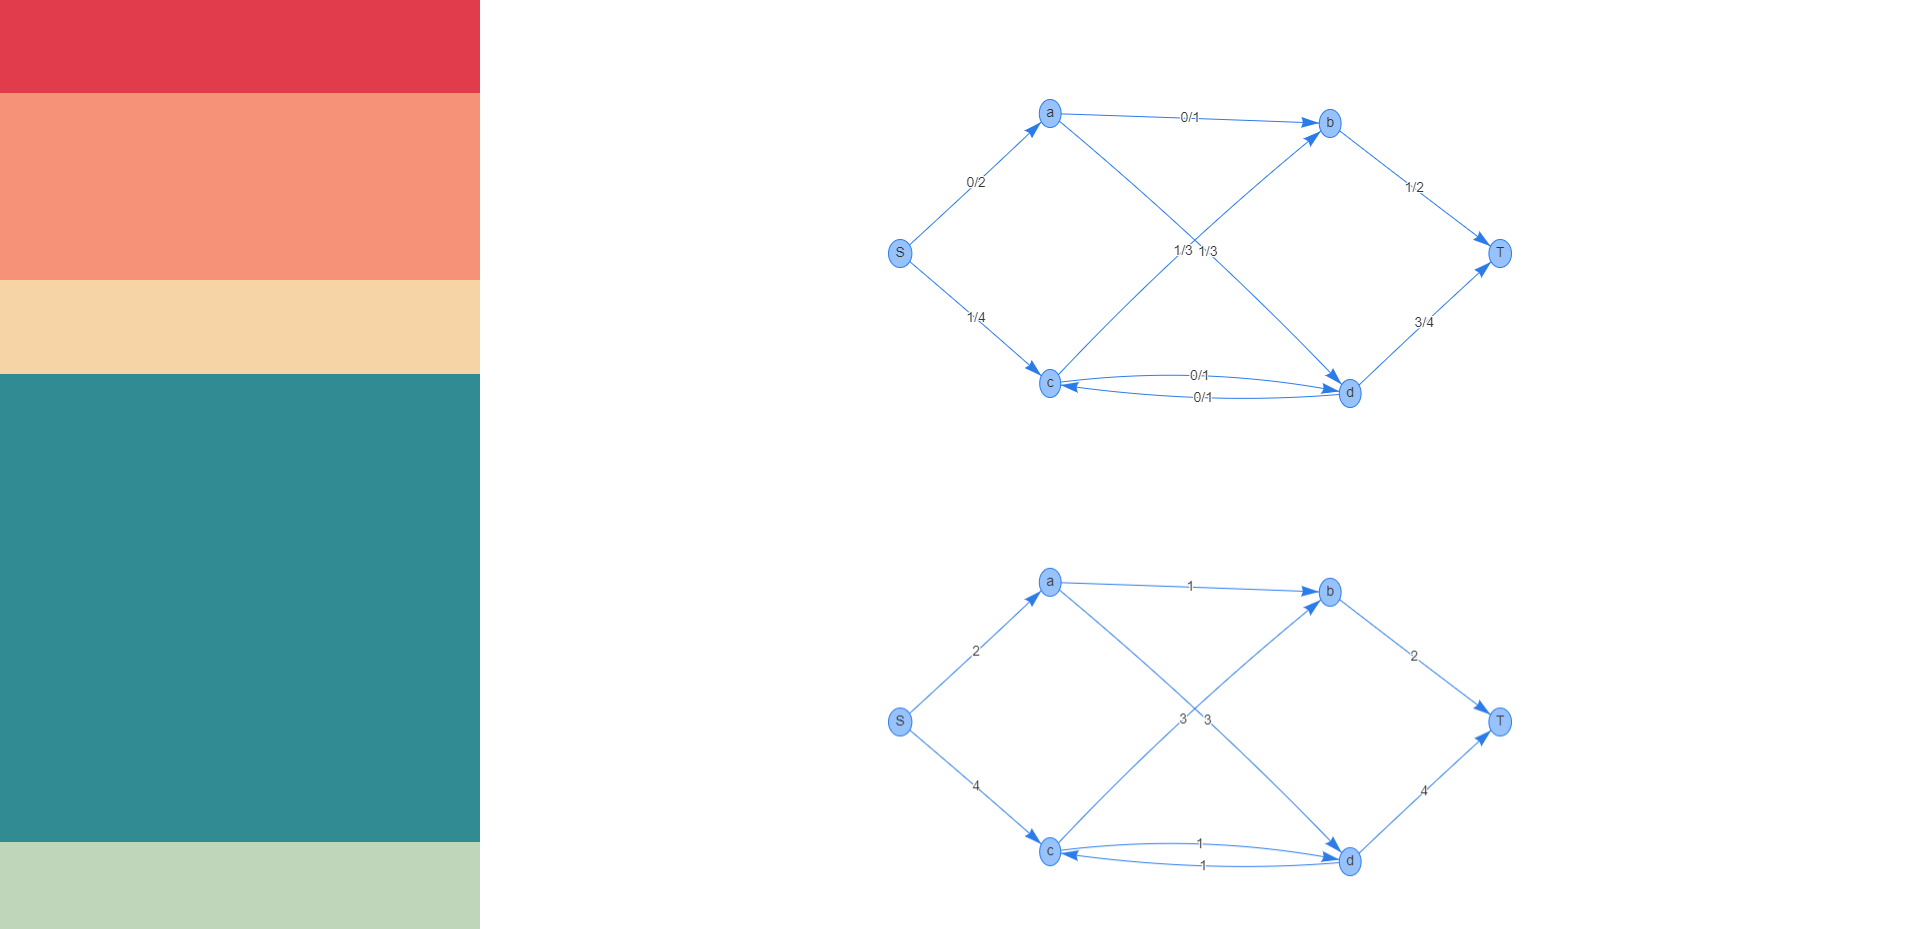
\includegraphics[width=\textwidth]{older-version.png}}
\caption{The initial design of the layout}
\label{fig:early-design}
\end{figure}

\begin{figure}[h!]
    \centering
    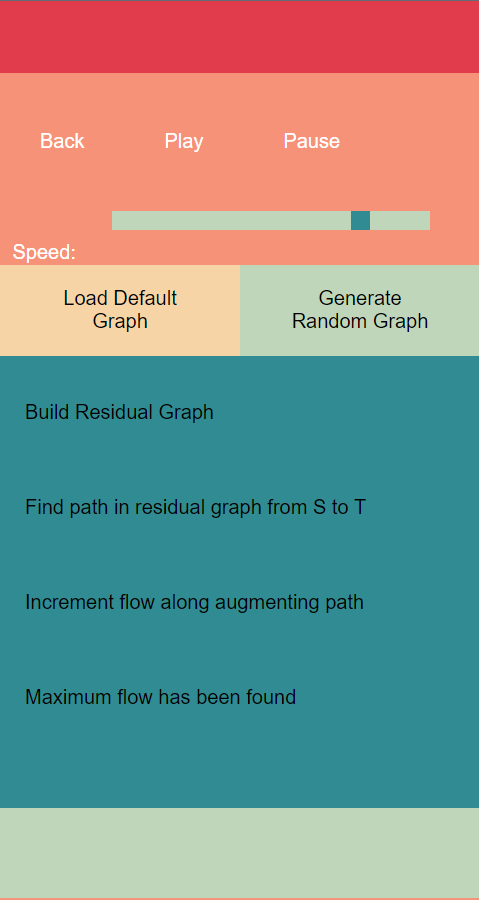
\includegraphics[width=0.3\textwidth]{infobar1.png}
    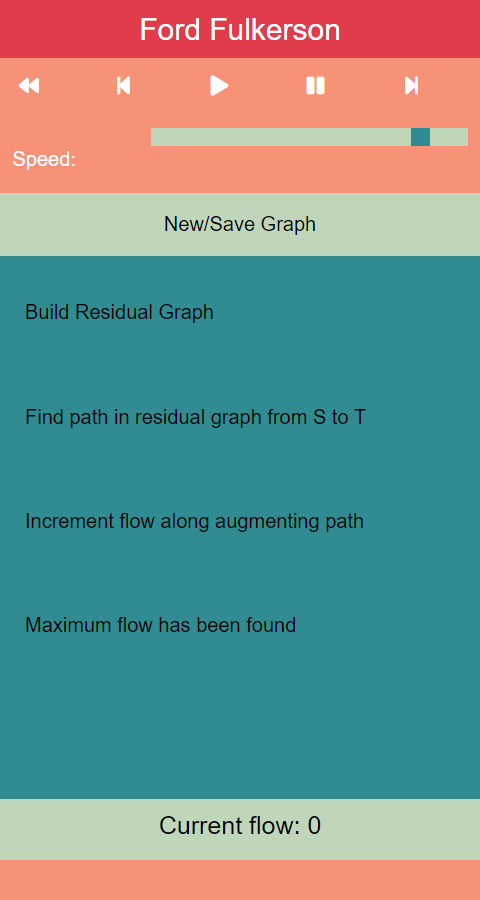
\includegraphics[width=0.3\textwidth]{infobar2.png}
    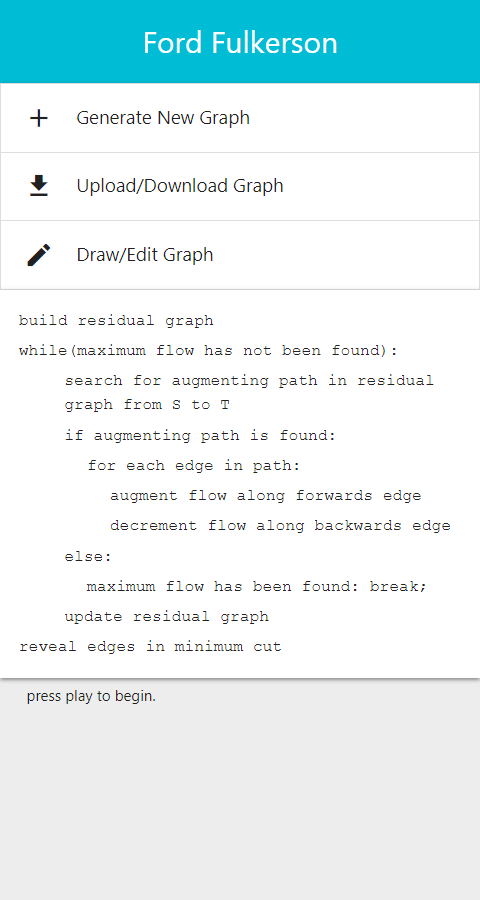
\includegraphics[width=0.3\textwidth]{infobar3.png}
    \caption{The design progression of the information bar}
    \label{fig:infobar-prog}
\end{figure}

As the product began to include more and more features unrelated to the animation, the space on the sidebar became limited and placing information in an intuitive, clear, and sensible way became infeasible (Centre of Figure \ref{fig:infobar-prog}). A redesign was implemented, taking great care to place each feature in a way that would be intuitive to the user. The greatest portion of the screen was still dedicated to the animation canvas, but a new row added beneath it containing the playback buttons, speed control slider, and flow counter. The former two were placed there to be similar to video player applications, and the flow counter stood alone to draw attention to it.

Updates to the information bar included a more intuitive placement of the network generation functions; while they are grouped in a collapsible accordion menu indicating relation, their purposes are all distinct and clear. The collapsible menu then allowed extra room for more detailed pseudo-code, and the execution trace placed below that. The user would now be able to collapse the unnecessary graph information while the animation runs, and focus on the algorithm details.

Additionally, a more cohesive colour theme was chosen: teal, with an orange accent to draw attention to important information (e.g. the highlighted line of pseudo-code (Figure \ref{fig:final-design}), among other things). To avoid confusion, the residual graph would not be revealed until the animation had begun. Iconography was used to replace instructions where possible.

\begin{figure}[h]
\centering
\fbox{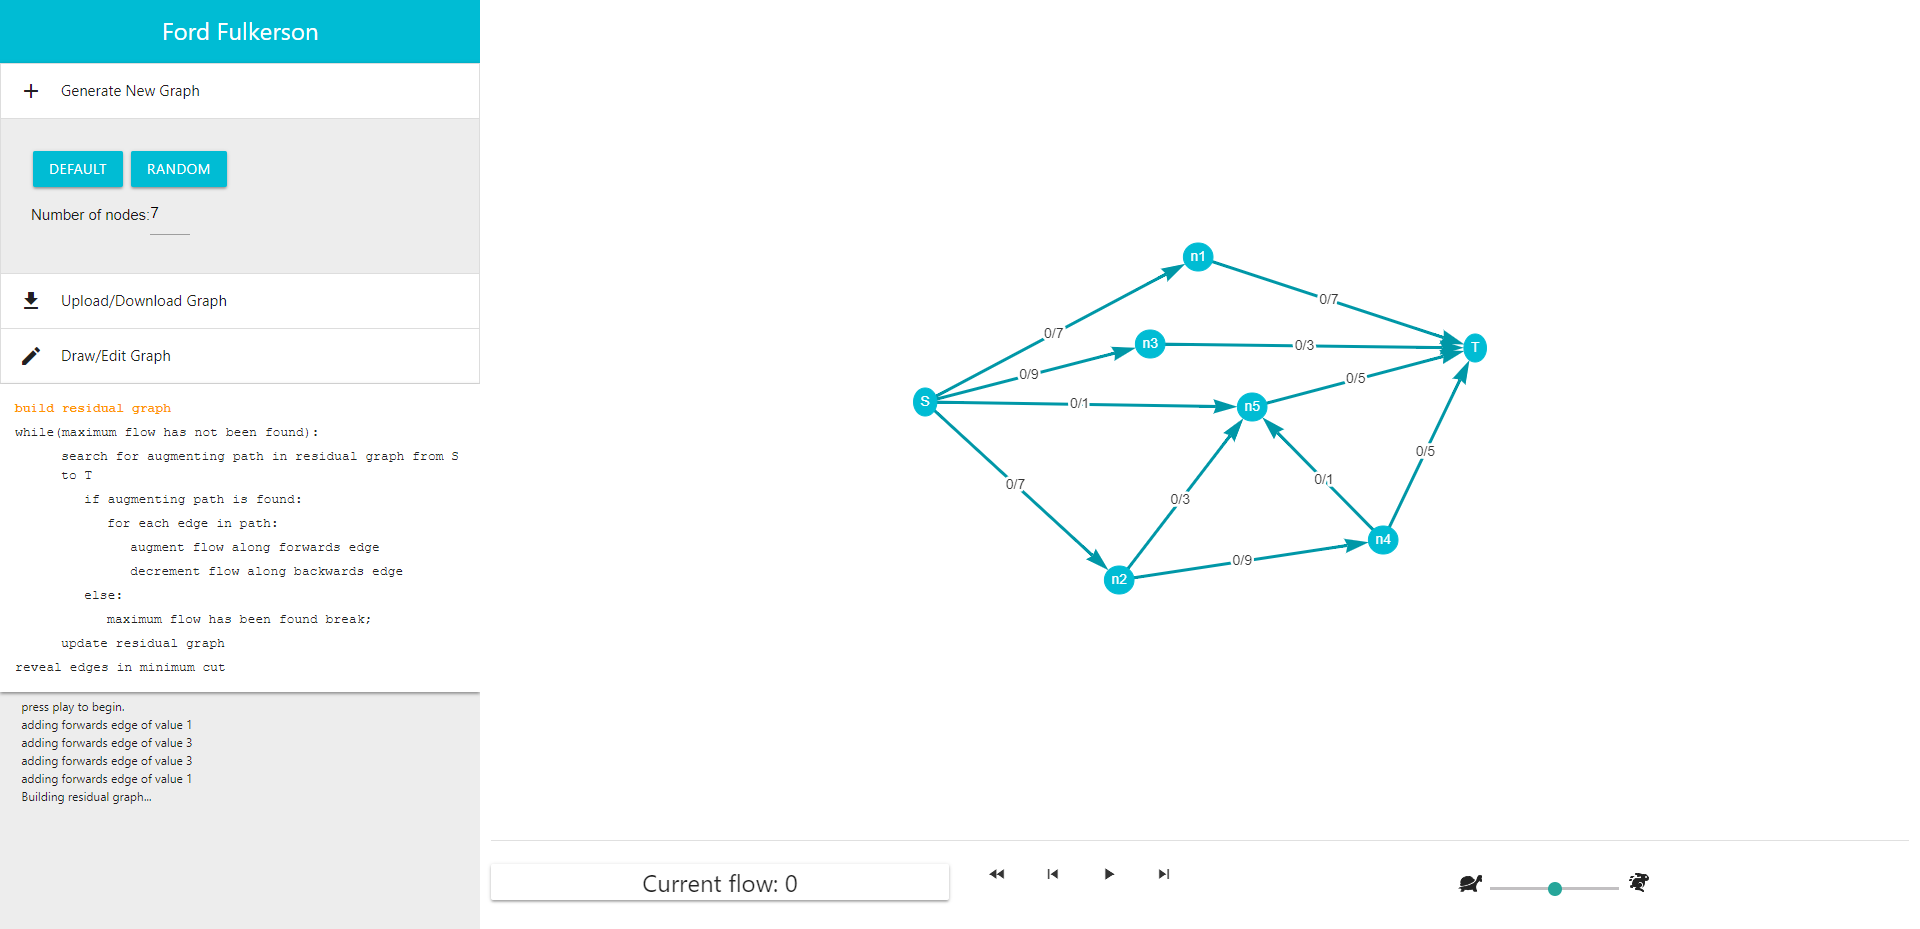
\includegraphics[width=0.9\textwidth]{current-design.png}}
\caption{The final product design.}
\label{fig:final-design}
\end{figure}

\newpage
\section{Animation}
There were two major areas to consider for the animation method. The first was the order in which the calculation of the algorithm and the execution of the animation should go in. Either the entire algorithm could be run and the animation prepared before anything was shown to the user, or the algorithm could be calculated during the animation. In order to fulfil the requirement of playback features most efficiently, the former was chosen. The second area was the data structure needed to store the information that this animation used, and what to include in the objects stored in the structure. This was decided early on in the design process, and proved robust enough to remain mostly unchanged throughout the project.

\subsection{Method}
The animation manipulates one edge at any time from either the top graph or the residual graph. The data stored is an array composed of objects called ``animation steps". Each object details the edge that is being changed, the action in which it is being changed (eg change of colour or label), and additional information such as which pseudocode line should be highlighted during that step. When the user presses play, the animation engine iterates through this array with the desired intervals, and the graphs change accordingly.

\begin{figure}[h]
    \centering
    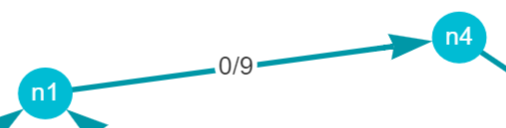
\includegraphics[width=0.3\textwidth]{animate1.png}
    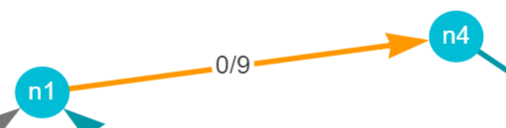
\includegraphics[width=0.3\textwidth]{animate2.png}
    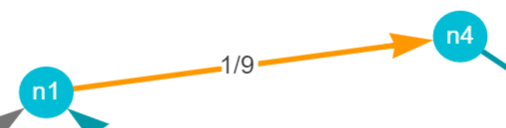
\includegraphics[width=0.3\textwidth]{animate3.png}
    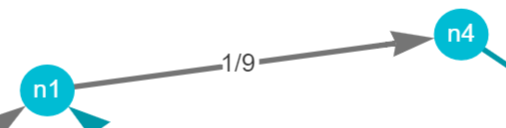
\includegraphics[width=0.3\textwidth]{animate4.png}
    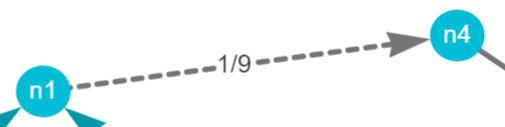
\includegraphics[width=0.3\textwidth]{animate5.png}
    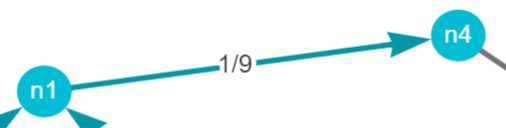
\includegraphics[width=0.3\textwidth]{animate6.png}
    \caption{Each stage of an edge in the top graph having flow incremented. The edge is highlight in orange, the label updated, highlighted in grey, dashed (as the residual graph is updated, not shown here), and then highlighted in its original colour.}
    \label{fig:my_label}
\end{figure}

In order to have a rewind function, whenever an animation step is executed it stores the previous state of its edge. When the user rewinds the animation, the animation traverses the array of animation steps backwards from the index it had reached, and restores each edge to its previous state.

\subsection{Styling}
// TODO how animation was designed to be clear.

\chapter{Implementation}
\section{Technology}
Due to the decision to create the product as a web-page, it was entirely written HTML, CSS, and JavaScript.
The javascript library $vis.js$ was used in both the calculations behind the algorithm and the graphical display of the networks. A different library $sigma.js$ was also considered, but the styling and flexibility options were more limited.
For the UI, materialize \cite{materialize} was used to create a familiar and unified feel to the design.

\subsection{vis.js}
A $vis$ Network \cite{network} is the object used to visualise the networks displayed, comprised of several modules that define specific aspects of the network, most notably the node and edge DataSets.
$Vis$ DataSets \cite{dataset} are key/value based structures used to store and manipulate the sets of nodes and edges that comprise each network. Each object in a DataSet has a unique identifier, used to access and manipulate it.
Node objects \cite{nodes} contain several options, including styling, manipulation, physics, and positioning. Edge objects \cite{edges} have similar properties, with additional options specifying the nodes that the edge connects.

In addition to the node and edge DataSets were options governing node layout, user interaction, and an interface for user manipulation. Networks are displayed graphically using an HTML element as a canvas.
\begin{comment}
TODO table of functions used frequently with DataSets

\end{comment}

\section{Network Generation}
One of the foremost tasks of implementation was to have a tool to create networks on which to run the Ford Fulkerson algorithm. First of all, a default network was needed for consistent testing. This was achieved by hard-coding an array of nodes with preset $x$ and $y$ values for a predictable layout (see Figure \ref{fig:xandy}), and an array of edges with predetermined capacities and connecting nodes.
\begin{figure}[h]
\centering
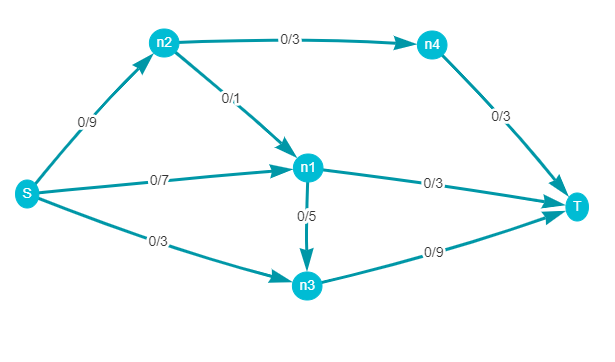
\includegraphics[width=0.47\textwidth]{xandy1.png}
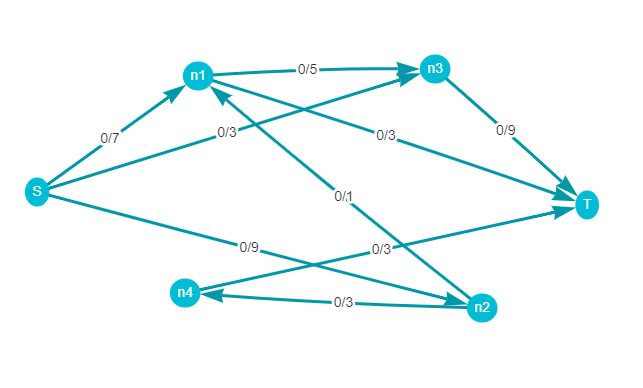
\includegraphics[width=0.47\textwidth]{xandy2.png}
\caption{How differing $x$ and $y$ values can drastically change the look of a graph}
\label{fig:xandy}
\end{figure}

\subsubsection{Random drawing} \label{randomise}
It was crucial to my requirements to be able to also randomly generate networks. However, these ``random" graphs would have to fit standards to still be a useful and clear tool for the display of the algorithm, as follows:
\begin{itemize}[noitemsep]
	\item The source must be the left-most node, and the sink the right-most
    \item Each node must have two edges, and be on a path from the source to the sink
    \item There must be no circular (i.e. from and to the same node) or parallel edges
    \item There should be no edges incoming to the source, or outgoing from the sink
    \item Nodes should not overlap
    \item Edge capacity should be between 1 and 10
\end{itemize}
The first requirement was implemented by initialising the source and sink with preset positions on the left and right of the canvas. The $x$ and $y$ coordinates for all other nodes are randomly assigned on creation. On rare occasions they can overlap, but this was mitigated by the $vis$ physics engine causing nodes to repel each other, or in the event of that failing, the user's ability to drag and place the nodes anywhere on the canvas.

The remaining nodes and edges are added by the following method:
\begin{enumerate}[noitemsep]
    \item Any two unconnected nodes would be connected to the sink ($T$). This ensures that $T$ has at least two incoming edges. Every unconnected node after that would be either connected to $T$, or any node already on a path to $T$. This continues until all nodes form a spanning tree. At the end of this stage, all the nodes with no incoming edges form a set ($A$).
    \item The next two edges generated would be from the source $S$ to any node $n$ from $A$. $n$ would then be removed from the set. This ensures that $S$ has at least two outgoing edges. Edges would then be added from $S$, or any node on a path from $S$, to any node in $A$ until $A$ was empty.
    \item Any edges not yet added would be added anywhere in the graph, provided they fitted the above criteria.
\end{enumerate}

\begin{figure}[h]
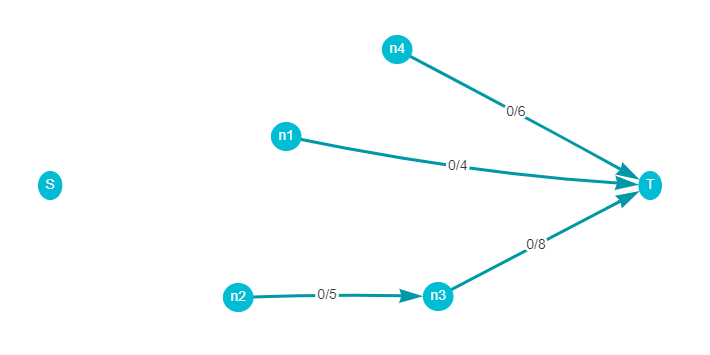
\includegraphics[width=0.49\textwidth]{step1.png}
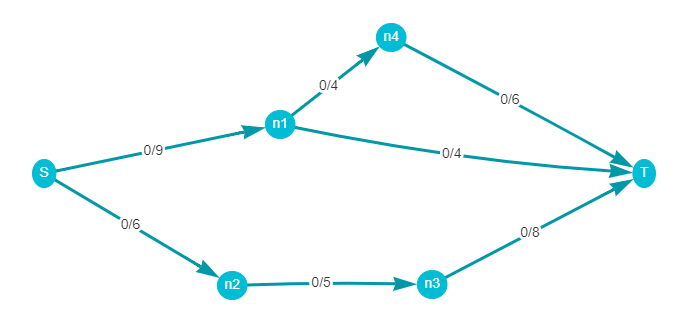
\includegraphics[width=0.49\textwidth]{step2.png}
\caption{Steps 1 and 2 of the random network generation}
\end{figure}

This approach ensured that there would be plenty of variety in the generated networks, while also providing a network that a user would be able to easily comprehend.
\subsubsection{User Inputs} \label{drawing}
For the uploading and downloading feature of the networks, the format of the files required careful thought. It must be detailed enough to preserve the layout of a network upon uploading it, but simple enough to understand with little instruction. An example of the file format is show below.

\begin{figure}[h]
    \centering
    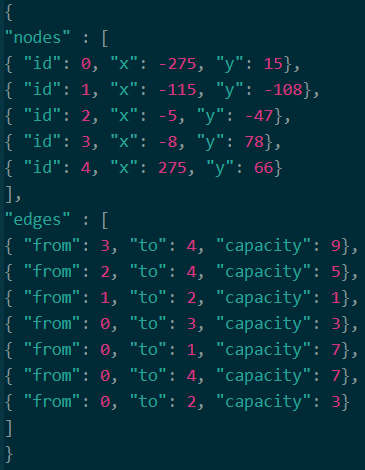
\includegraphics[width=0.25\textwidth]{json-graph-text}
    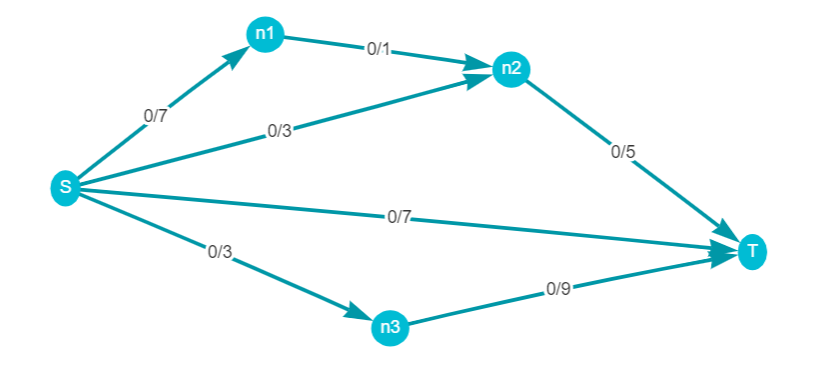
\includegraphics[width=0.7\textwidth]{json-graph-pic}
    \caption{\label{fig:json-graph}The json format for a small graph, and its graphical representation}
\end{figure}

The type of file chosen was json, in order to work efficiently with JavaScript, and the data stored with two arrays of nodes and edges. Each node must have an id, with the node with id = 0 being the source $S$, and the node with id = $N$ being the sink $T$, where $N$ is the number of nodes. The $x$ and $y$ values for nodes are optional; if not supplied, the node will be assigned a random coordinate. It is crucial to most of the calculations involving graph data that the node ids are in consecutive order. Each edge would have 3 parameters, all compulsory. The two nodes that the edge connected ``$from$" and ``$to$", and the capacity of that edge.

Downloading a graph would write a representation of the graph currently showing on the interface, and download it to the user's file system. If a file was uploaded, it would first be parsed to check for formatting errors, and then undergo a series of checks to ensure it was a correctly written graph. If there were any errors found in the file, and alert would be shown to user detailing the error.

\section{Algorithm}
\subsection{Graph data}
The Ford-Fulkerson algorithm in this project required two networks: the main (top) graph and the residual graph. In the implementation there were four networks stored, two for display, and two for the calculation of the algorithm. This is so that all the data for the algorithm could be calculated before the animation began, independent from the display. This section will focus exclusively on the algorithmic networks.

As previously stated, a network is made up of two $vis$ DataSets, nodes and edges. Both graphs share the same set of nodes, but have distinct sets of edges. In addition to these data structures each graph has an adjacency matrix representation ($topAdjMatrix$ and $resAdjMatrix$), where the cell between two connected nodes contains the unique ID of the edge connecting them. The ID of an object in a DataSet provides access to it with the $get()$ function, allowing its manipulation. The additional matrix representations hugely improved efficiency at several points of the algorithm.

\subsection{Building/updating residual graph}

Building the residual graph the first time copied each edge in the top graph to the residual graph with a weight of the edge's capacity, as no edge in the top graph could have a flow greater than 0. After each instance of the flow increasing, the residual graph would be updated along the augmenting path.

Updating the residual graph would occur after each edge of the augmenting path is incremented or decremented. The path is represented with an array of nodes that it traverses, from 0 to T, so each edge in the path can be accessed by taking two consecutive nodes, `$from$' and `$to$'. The `$capacity$' and `$flow$' of each edge in the top graph is used in the calculation, as are the `$forwards$' and `$backwards$' edges in the residual graph. The forwards edge goes in the direction of the augmenting path ($resAdjMatrix[from][to]$), and the backwards edge in the opposite direction ($resAdjMatrix[to][from]$).

\lstset{numbers=left}
\begin{lstlisting}
if(augmenting && (capacity - flow > 0)){
  update forwards edge label to (capacity - flow);
} else if (decrementing && (flow > 0)){
  update forwards edge label to flow;
} else {
  if((oppEdge = topAdjMatrix[to][from]) exists){
    oppFlow = getFlow(oppEdge);
    oppCap = getCapacity(oppEdge);
    if(augmenting and (oppFlow > 0){
      update forwards edge label to oppFlow;
    } else if (decrementing and (oppCap - oppFlow > 0)){
      update forwards edge label to (oppCap - oppFlow);
    }
  } else {
    remove forwards edge;
  }
}

if(backwards edge exists){
  if(augmenting) {
    update backwards edge label to flow
      or add backwards edge with label flow
  } else {
    update backwards edge label to (capacity - flow)
     or add backwards edge with label (capacity - flow)
  }
}
\end{lstlisting}

// TODO some graphical examples of it in action

This method of updating the residual graph leaves it updated such that there are no parallel edges. In the case of having two possible edges in the same direction, the algorithm will simply pick one. This makes the step at line 6 crucial in preventing a bug that removes an edge where it is still required. \label{edge-rem-bug}

// TODO graphical example of this bug

\subsection{Finding augmenting path and minimum capacity}
The augmenting path was found using a breadth-first search algorithm, shown below:
\begin{lstlisting}
findPath() {
  set each node's parent to itself;
  Queue.push(S);
  while(Queue.length > 0){
      current = Queue.shift();
      for(each node current connects to){
        if(node hasn't been visited){
          node.parent = current;
          Queue.push(node);
  } } }

  if(T.parent == T){
    return null;
  } else {
    path = [];
    current = T;
    while(current != S){
      path.push(current);
      current = current.parent;
    }
  }
  return path.reverse();
}
\end{lstlisting}
\begin{figure}[h]
    \centering
    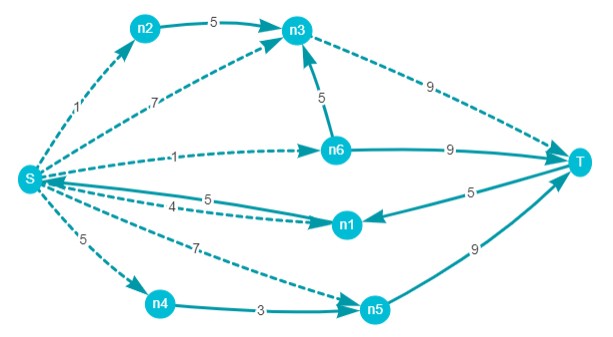
\includegraphics[width=0.6\textwidth]{bfs.png}
    \caption{Searching for a path in the residual graph. The edges being searched are shown dashed.}
    \label{fig:my_label}
\end{figure}

Once the path had been found, the minimum capacity of the path `m' had to be calculated. This is the value of the edge with the smallest amount of remaining capacity, and therefore the largest amount of flow that could be augmented along the path. A variable `minCap' would be compared to the available capacity of each edge. If minCap was greater than this capacity then it would be set to the value of the capacity.
\subsection{Augmenting/decrementing edges}
To represent the capacity and flow of a particular edge, the label property of an edge was assigned a string of the form ``$x/y$" where $x$ is the flow and $y$ is the capacity. There were three functions used throughout nearly every step of the algorithm: $getCapacity$, $getFlow$, and $setFlow$. Each of these took the label string and either returned the capacity, flow, or a new label.

\begin{lstlisting}
m = getMinimumCapacity(path);
for(edge in path) {
  if(edge direction == forwards) {
    edge flow = edge flow + m
  } else if(edge direction == backwards) {
    edge flow = edge flow - m
  }
}
\end{lstlisting}

Determining the direction of the flow was initially done by using the top graph's adjacency matrix (topAdjMatrix). A function $getEdgeData$ would take the `from' and `to' node ids, and return an object containing the edge id (in the top graph) and its direction. If $topAdjMatrix[from][to]$ was found to exist, then the direction would be forwards (represented as 1), but if that was null and $topAdjMatrix[to][from]$ existed, the direction would be backwards (0). However, this overlooked the possibility of there being two edges between `from' and `to', as then the forwards edge could be selected when the other was correct.

This was fixed by adjusting the residual graph to include a tag on each newly added backwards edge, during the updating of the residual graph. Then instead of checking the direction of the edge in the top graph, the tag would be checked. If true, the direction would be backwards. If null, forwards.

\subsection{Finding the minimum cut}
To find the minimum cut, a set of nodes $A$ is composed of the source node $S$ and all nodes that $S$ can access via the residual graph, after the algorithm has completed. The set of nodes $B$ is all other nodes in the graph. The minimum cut $C$ is the set of edges in the top graph from any node in $A$ to any node in $B$.

\begin{figure}[h]
    \centering
    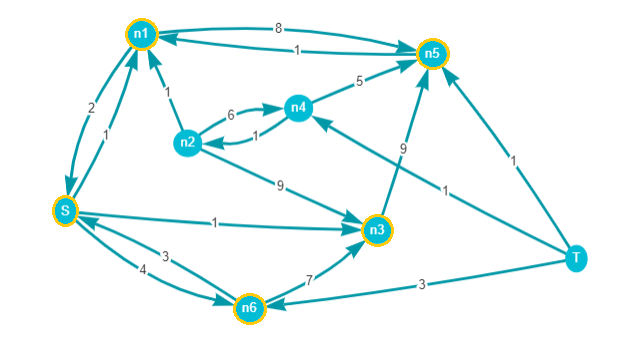
\includegraphics[width=0.45\textwidth]{res_min_cut.png}
     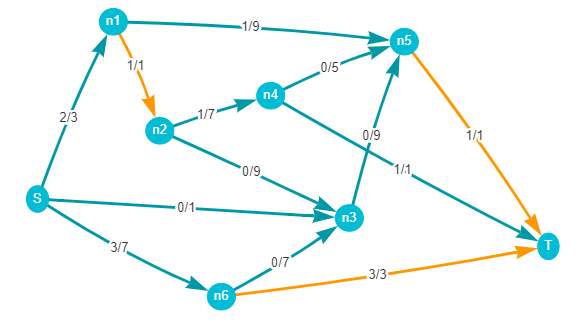
\includegraphics[width=0.45\textwidth]{top_min_cut.png}
    \caption{The residual graph with set $A$ highlighted, and the top graph with minimum cut $C$ highlighted}
\end{figure}
\begin{figure}[h]
    \centering

\end{figure}

\section{Animation}
\subsection{Animation Steps}
All the detail in one animation step

How different animation steps are made in practice

\subsection{Animation Engine}
How the animation engine processes the information

What does play state mean? How it affects the animation engine.

\section{Code Organisation}

\chapter{Evaluation}
\begin{comment}

What did we do? (state precisely how you went about evaluation; methods, apparatus, and procedure such that someone else could reproduces your experiment and get same data)
What data did we get? (present summary of results)
Analyse data. (graphs, stats or tables which draw out evidence that answers your questions from the data)
Draw conclusions. (answer the questions you asked precisely, referring to your analysis)
\end{comment}
The purpose of the evaluation was to answer the following questions:
\begin{itemize}
    \item Is the implementation of the Ford-Fulkerson algorithm correct?
    \item Is the design of the application intuitive to use?
    \item Does the application present the algorithm in a way that strengthens understanding?
\end{itemize}
\section{Correctness testing}
The implementation of the algorithm was tested using the Min-cut/Max-flow theorem, which states that the maximum flow of a network is equal to the sum of the capacities of the minimum cut of the network.

The test used is shown below, simplified:
\begin{lstlisting}
generateRandomGraph();                  // generates a random network with N nodes
FFMaxFlow = fordFulkerson();        // Runs Ford-Fulkerson algorithm on this network,
                                        // and returns maximum flow found
cut = findMinimumCut();
cutMaxFlow = removeEdgesInCut();    // Removes edges in minimum cut from network,
                                            // and returns the sum of their capacities
path = findPath();      // Attempts to find a path from S to T
if(path != null){
    min-cut is invalid, test has failed
}
if(FFMaxFlow != cutMaxFlow) {
    max-flow min-cut theorem shows test has failed
} else {
    test has passed
}
\end{lstlisting}

A function $testFF$ ran the test. It was used in two ways:

\begin{enumerate}
    \item $testFF(n, iter)$ would take a value for $N$ ($n$) and a value for the number of iterations ($iter$). It would then execute the test $iter$ times, and then print out the percentage of incorrect tests at completion.
    \item  $testFF()$ would run until failure, at which point it would print out the network data used in the failed test.
\end{enumerate}

The former way was used to uncover the presence bugs in the implementation, as subtle or rare bugs could be discovered with higher values of $N$ and more iterations. The latter was used to debug them with smaller sets of data (eg $N \approx 5$). When a failed test returned, the data from it could be entered into the application and the animation could be run to determine the cause of failure.

When the correctness testing was first implemented, it revealed that the implementation was incorrect 0.05\% of the time on average. A bug partially behind the failure rate was caused during the updating of the residual graph, which was then fixed (Section \ref{edge-rem-bug}).

Failure rate then decreased, but was still non-zero. The cause of this was also from the residual graph being updated, in rare cases when a backwards edge would be used multiple times. Once this was fixed, any value of $N$ or iterations would return no failed tests. This satisfied the first of the questions to be answered by the evaluation.

\begin{figure}[h]
    \centering
    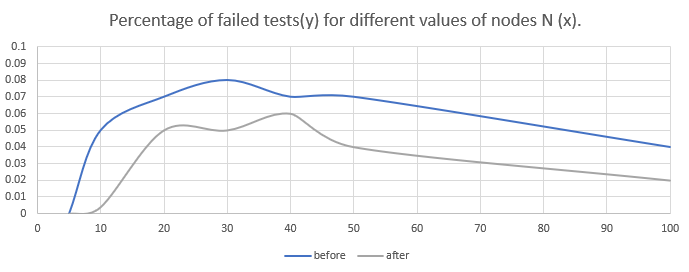
\includegraphics[width=\textwidth]{correctness.png}
    \caption{The application was tested with varying numbers of nodes from 5-100 with 10000 iterations for each value. This figure shows the drop in failure rates when the former bug was removed.}
    \label{fig:my_label}
\end{figure}

\section{User evaluation}
To evaluate the UI and effectiveness of the animation, usability tests were conducted on 8 participants, all of which had had prior experience of the Ford-Fulkerson algorithm in their courses. The evaluation was split into two sections. The first section covered a series of tasks to create graphs, and the second section covered the animation and its effectiveness. To begin the evaluation, participants were asked to rate their understanding of the Ford-Fulkerson algorithm on a scale of 1 to 10, where 1 is no understanding at all and 10 is complete understanding.

\subsection{Section 1: Graph generation}
After this, the first section of the evaluation began. The participant was asked to complete three tasks:
\begin{enumerate}
    \item Generate a random graph with 8 nodes
    \item Download the graph from the previous task, and add a new edge (in the file) between any two nodes. Upload this altered graph.
    \item Draw this example graph (Figure \ref{fig:eval-graph}), and save it.
\end{enumerate}

\begin{figure}[h]
    \centering
    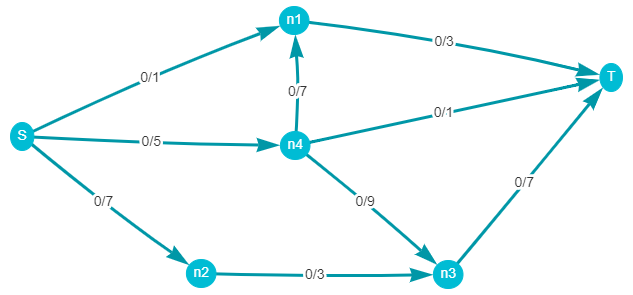
\includegraphics[width=0.6\textwidth]{graph-eval.png}
    \caption{The example graph evaluation participants were asked to draw.}
    \label{fig:eval-graph}
\end{figure}

\begin{figure}[h]
    \centering
    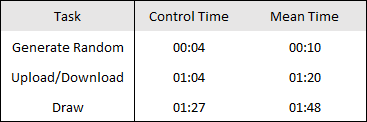
\includegraphics[width=0.6\textwidth]{task-time-table.png}
    \caption{Comparing the mean times to complete the three tasks.}
    \label{fig:timed-tasks}
\end{figure}

Each task was timed, and any critical or non-critical errors were noted. The tasks were designed so that the user would have to explore each feature of graph generation. The purpose was to check that the design of each feature was intuitive. I timed myself performing each of these tasks to compare the results to, shown under ``Control Time" in Figure \ref{fig:timed-tasks}.

There were no critical errors for any tasks, all participants were able to complete their tasks within a few minutes. Three Participants experienced non-critical errors with Downloading a graph as a json file and altering it:

\begin{itemize}[noitemsep]
    \item Added a duplicate edge.
    \item Trailing comma, and added edge to non-existent node.
    \item Trailing comma.
\end{itemize}

Four participants encountered non-critical errors with drawing a new graph:

\begin{itemize}[noitemsep]
    \item Accidentally cleared progess. The `enter' button clears canvas when nothing selected.
    \item Tried to edit edge capacity, not possible.
    \item Not clear on ``capacity" meaning (entered 0/6 when prompted).
    \item Could not find ``draw graph" right away.
\end{itemize}

After these tasks, the following qualitative questions were asked:
\begin{enumerate}[noitemsep]
    \item Was there anything you liked about generating a new graph?
    \item Was there anything you disliked about generating a new graph?
    \item Do you have any recommendations for graph generation?
\end{enumerate}

Here are the results below:
\begin{figure}[h]
    \centering
    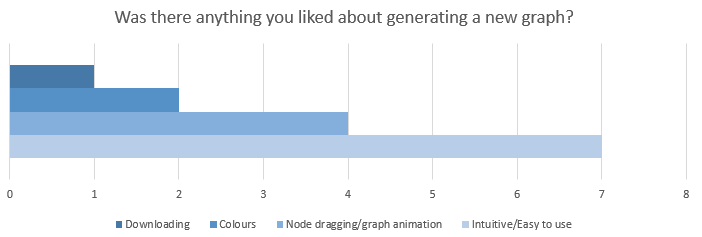
\includegraphics[width=0.9\textwidth]{graph-qual1.png}
    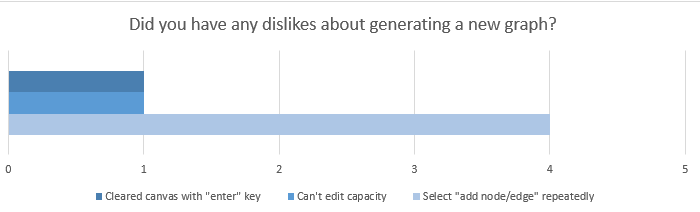
\includegraphics[width=0.9\textwidth]{graph-qual2.png}
    \caption{Common categories of candidate's opinions, grouped by rate of occurrence.}
    \label{fig:my_label}
\end{figure}

Comments regarding candidate's positive opinions on graph generation often mentioned that it was intuitive and easy to use, with one participant stating that they "didn't have to read much" and another saying there were "no extra distractions". Participants also expressed a fondness for the ``wiggly" appearance of the edges when nodes are dragged: this is categorised above under graph animation.

The most common aspect that candidates disliked about graph generation was that to add multiple nodes or edges when drawing graphs, the ``add node" or ``add edge" button must be pressed after each addition.

This was brought up twice when participants were asked if they had any recommendations for graph generation. In addition, one participant recommended clearer instructions for the upload/download feature, pointing out that the json example was not correctly formatted json. Edge capacity was mentioned twice in the recommendations, one suggesting it should be entered via a pop-up rather than an alert, and another candidate wishing to edit the capacity of an edge without replacing it.

\subsection{Section 2: Animation}
In this section the participant was asked to: "Run the animation for the current graph. Utilise the playback features as much as you need to try and best understand the algorithm. This is not timed.".

After they stated that they had completed this task, the following questions would be asked:

\begin{enumerate}[noitemsep]
    \item What edges are included in the minimum cut?
    \item What is the maximum flow of this graph?
    \item How did you determine the maximum value?
    \item What was the last augmenting path found in the animation?
\end{enumerate}

Each of the answers could be answered by using different components shown on the screen. The answers to questions 1, 2 and 4 were able to be quantified into correct, partially correct (for questions 1 and 4), or incorrect. Question 3 was to test that the flow counter component was clear. Question 4 was designed to make the participant check the execution trace for the answer.
\begin{figure}[h]
    \centering
    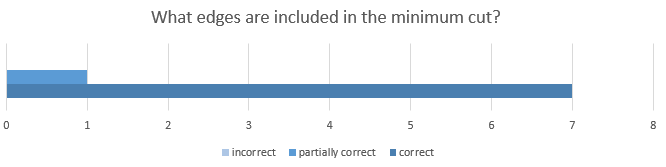
\includegraphics[width=0.9\textwidth]{cpci1.png}
    \label{fig:my_label}
\end{figure}

The participant who had a ``partially correct" response to the edges in the minimum cut also stated that they did not know at all what a minimum cut was.

\begin{figure}[h]
    \centering
    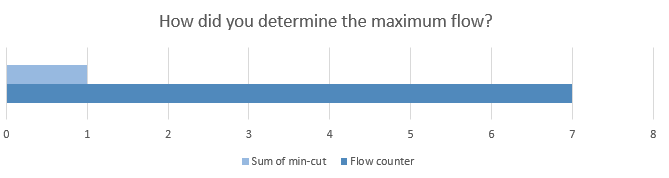
\includegraphics[width=0.9\textwidth]{cpci2.png}
    \label{fig:my_label}
\end{figure}
\begin{figure}[h]
    \centering
    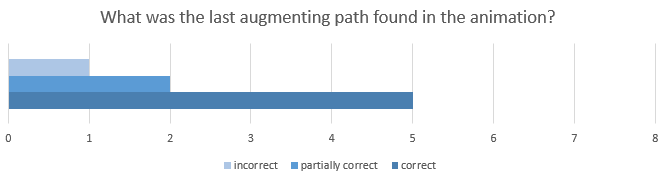
\includegraphics[width=0.9\textwidth]{cpci3.png}
    \label{fig:my_label}
\end{figure}
Participants were advised that the answer to the last augmenting path on the screen. Answers marked ``partially correct" had difficulty locating the execution trace line.

\newpage
The participants understanding of the animation was then evaluated by rating the following statements on a scale from 1 to 5, where 1 is totally disagree, and 5 is totally agree.

\begin{figure}[h]
    \centering
    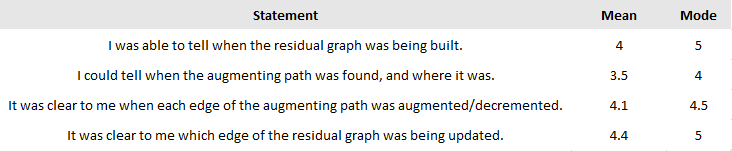
\includegraphics[width=\textwidth]{statements.png}
    \caption{The statements that each participant was asked to rate on a scale from 1 to 5, and the mean and mode of their responses.}
    \label{fig:my_label}
\end{figure}

Then the following qualitative questions were asked:
\begin{enumerate}[noitemsep]
    \item Were there any parts of the animation that weren’t clear to you?
    \item Are there any features of the playback/animation that you liked?
    \item Are there any features of the playback/animation that you disliked?
    \item Do you have any recommendations about the animation?
\end{enumerate}
\begin{figure}[h]
    \centering
    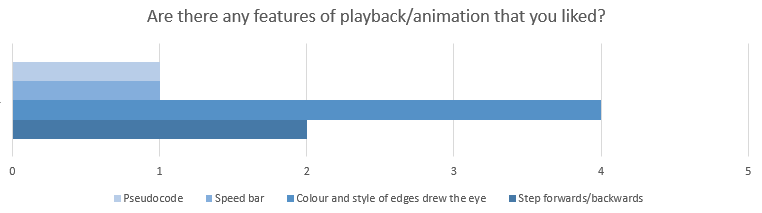
\includegraphics[width=\textwidth]{graph-qual3.png}
    \caption{Caption}
    \label{fig:my_label}
\end{figure}
\begin{figure}[h]
    \centering
    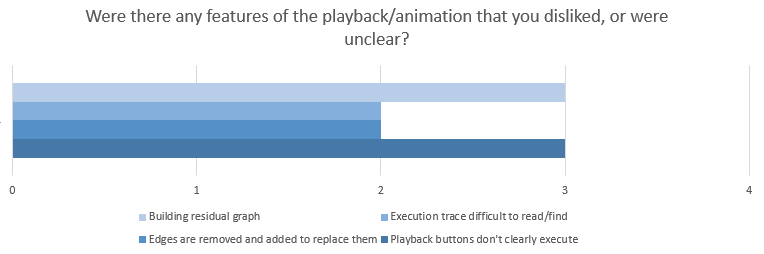
\includegraphics[width=\textwidth]{graph-qual4.png}
    \caption{Caption}
    \label{fig:my_label}
\end{figure}

Recommendations for animation:
\begin{itemize}[noitemsep]
    \item print when button is clicked; buttons need more feedback
    \item select a traceback line to go back in animation; happen on one graph
    \item Change label text style to draw more attention to change of flow
    \item would like to jump to very start
    \item no feedback for every action in UI
    \item execution trace isn't obvious
    \item execution trace more obvious
    \item brighter colour on top when building res graph
\end{itemize}

\newpage
Finally, participants were asked to re-evaluate their understanding of the Ford-Fulkerson algorithm as in the start of the evaluation. They were also given the opportunity for any additional comments on the project.

\begin{figure}[h]
    \centering
    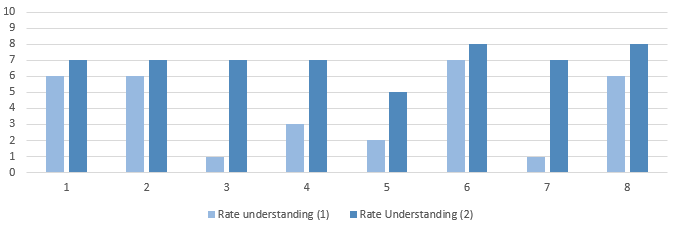
\includegraphics[width=\textwidth]{understanding.png}
    \caption{Caption}
    \label{fig:my_label}
\end{figure}
\section{Discussion}


\chapter{Conclusion}
\begin{comment}
Summarise the whole project for a lazy reader who didn't read the rest.
Summarise briefly and fairly. Indicate what future work could be done, but remember: you won't get credit for things you haven't done.
\end{comment}

\begin{thebibliography}{}
\bibitem{alg-animation}http://www.doc.ic.ac.uk/~nd/surprise\_95/journal/vol2/ad1/article2.html
\bibitem{algomation}http://www.algomation.com/algorithm/prim-minimum-spanning-tree
\bibitem{visualgo}https://visualgo.net/en/maxflow
\bibitem{usfca}www.cs.usfca.edu/~galles/visualization/BFS.html
\bibitem{network}http://visjs.org/docs/network/
\bibitem{dataset}http://visjs.org/docs/data/
\bibitem{nodes}http://visjs.org/docs/network/nodes.html
\bibitem{edges}http://visjs.org/docs/network/edges.html
\bibitem{materialize}https://materializecss.com/about.html

\end{thebibliography}

\end{document}
